\documentclass[11pt,a4paper]{article}

\usepackage[
    top    = 1in,
    right  = 1.5in,
    bottom = 1in,
    left   = 1.5in]{geometry}
\usepackage[utf8]{inputenc}
\usepackage[english]{babel}
\usepackage[T1]{fontenc}
\usepackage{lmodern}

\usepackage{amsmath,amssymb,amsfonts,float,subcaption,mathtools}

\title{Vision and Image Processing\\Assignment 4}
\author{Malte Stær Nissen    \\ \texttt{tgq958} \and
        Benjamin Braithwaite \\ \texttt{cpg608}}

\begin{document}
\maketitle

\section{Kanade-Lucas-Tomasi (KLT) tracker}

\section{Testing}
%
We test our tracker on the provided dudekface image sequence. Selected frames with the tracked features are shown in Figure \ref{fig:tracker_dudekface}.
%
\begin{figure}[H]
\centering
\begin{subfigure}{0.45\textwidth}
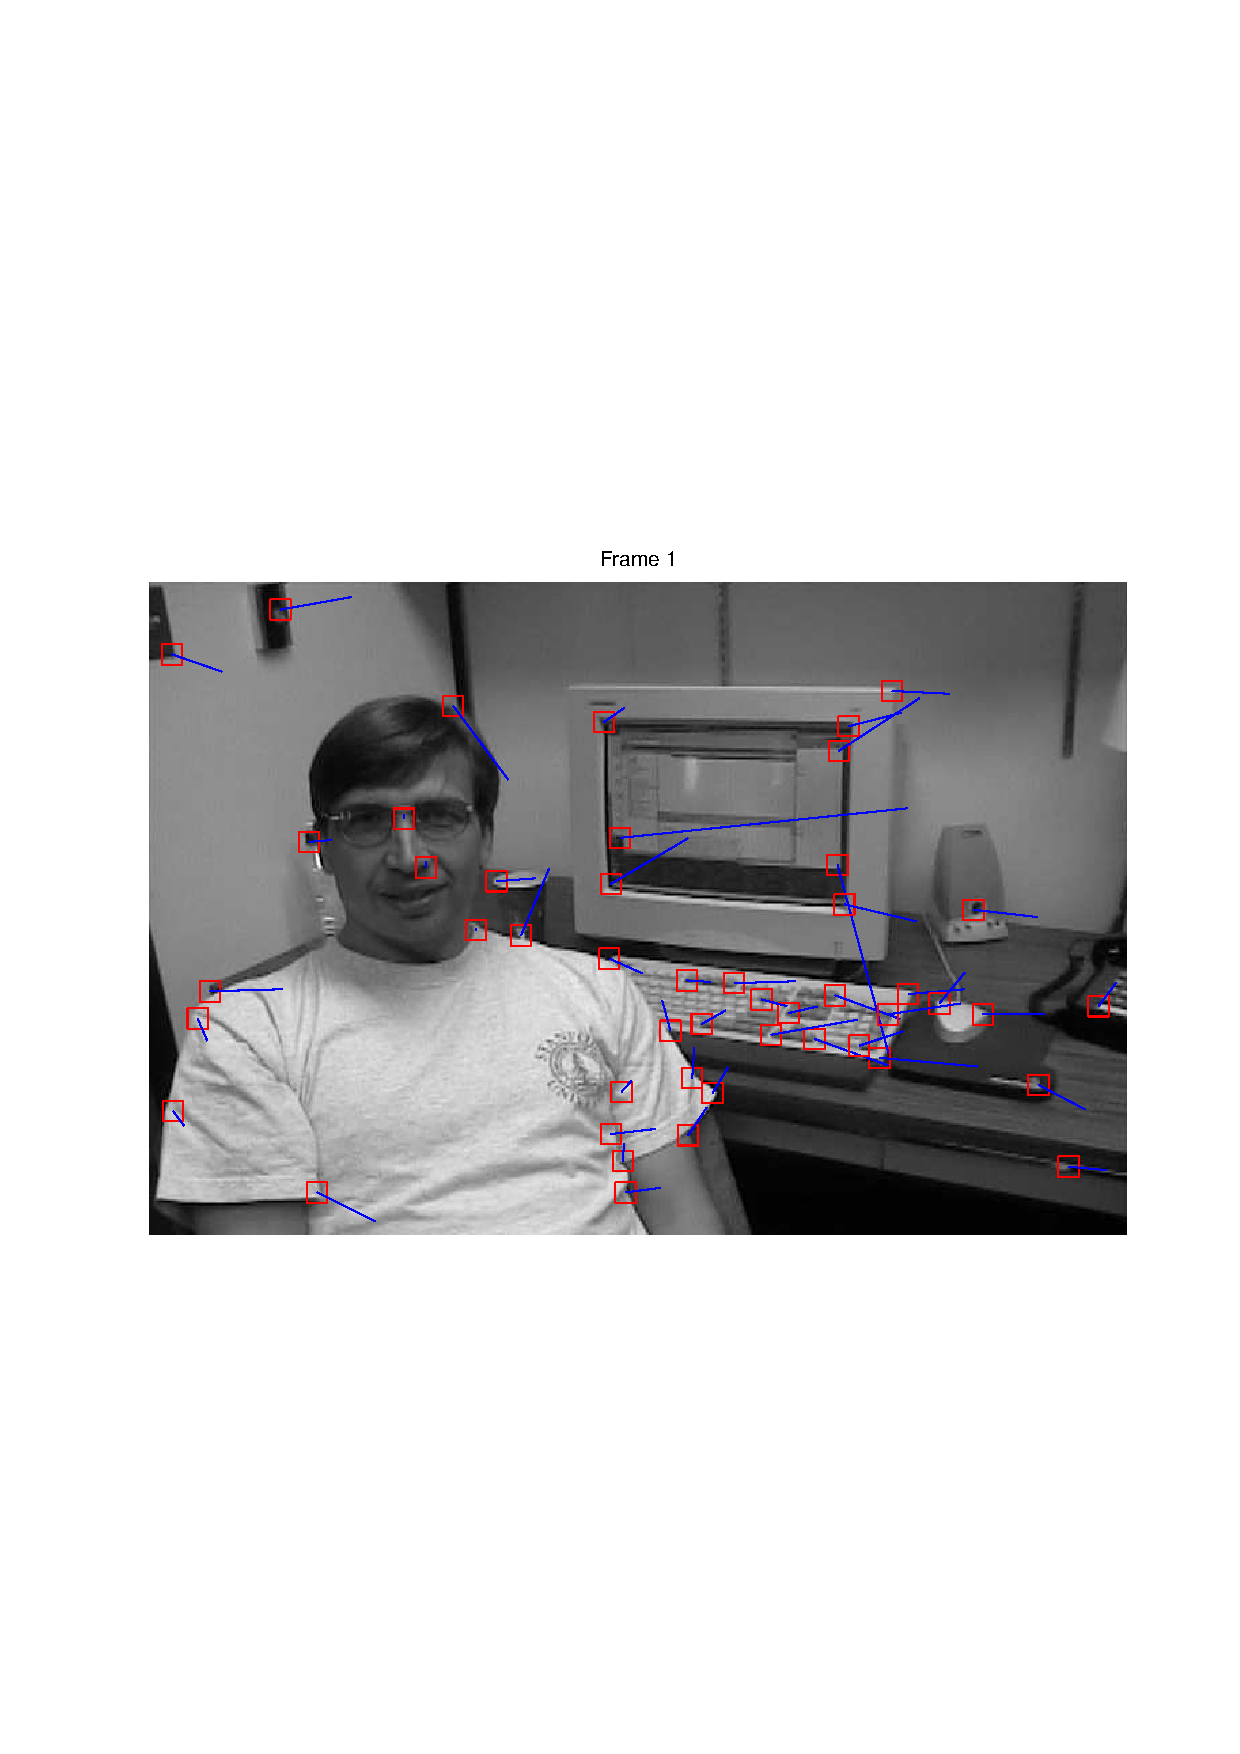
\includegraphics[scale=0.4,trim={120 250 0 250}]{img/tracker_dudekface_1.pdf}
\end{subfigure}
\begin{subfigure}{0.45\textwidth}
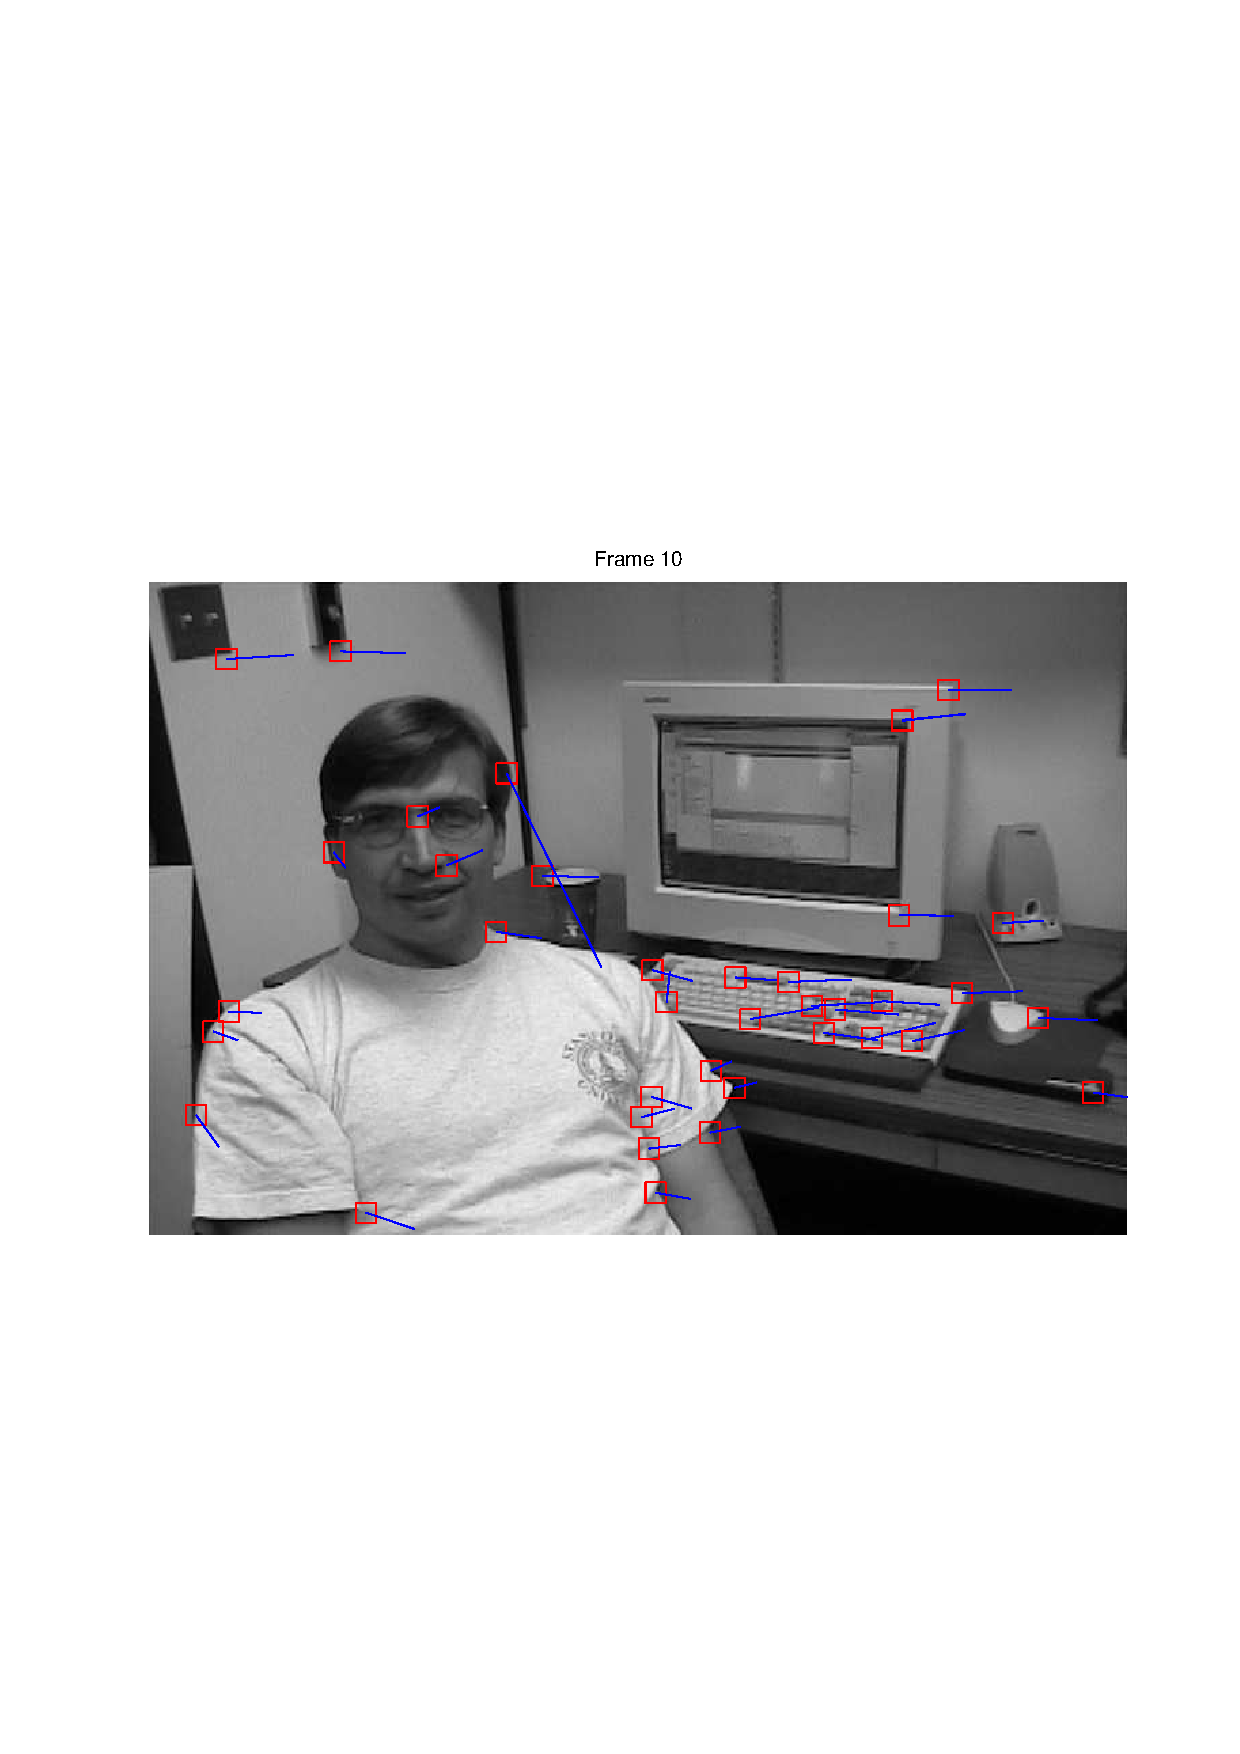
\includegraphics[scale=0.4,trim={70 250 0 250}]{img/tracker_dudekface_10.pdf}
\end{subfigure}
\begin{subfigure}{0.45\textwidth}
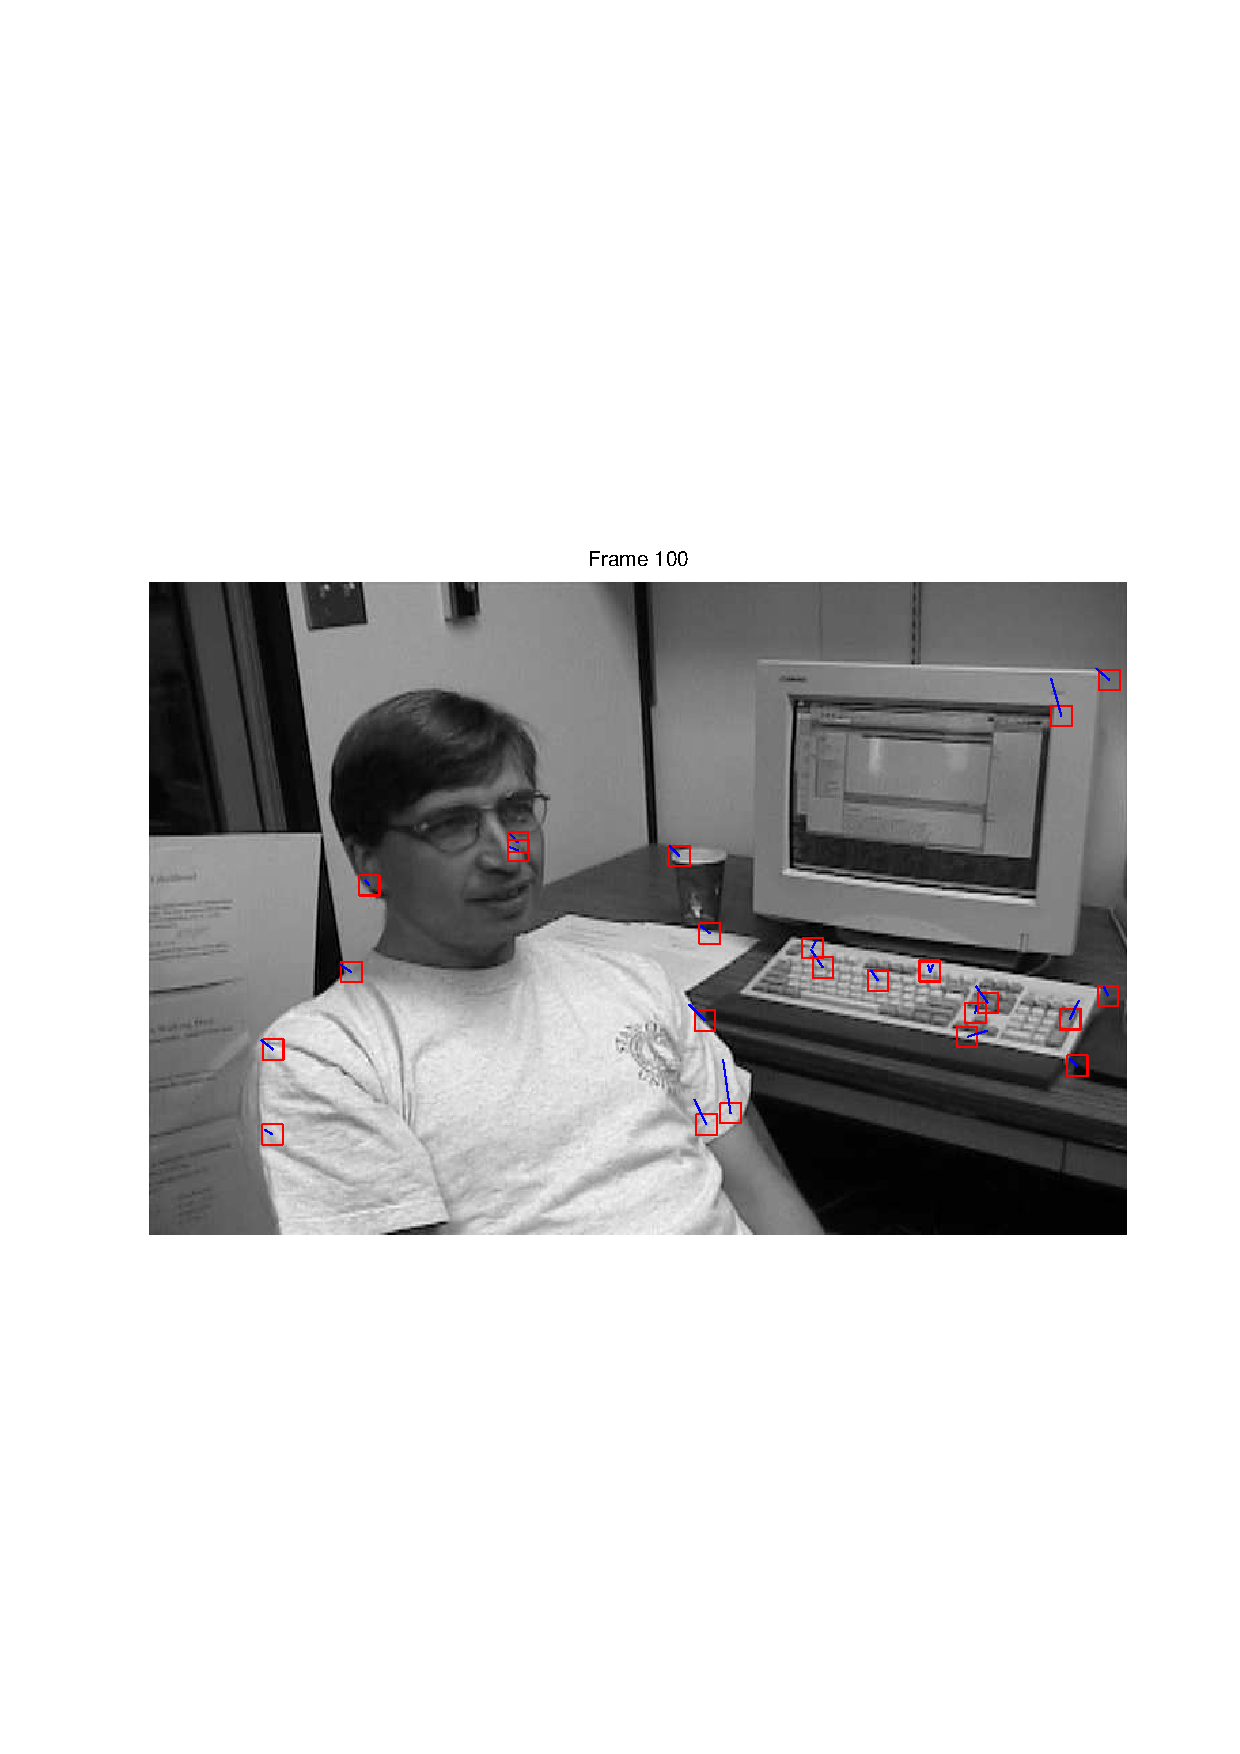
\includegraphics[scale=0.4,trim={120 250 90 250}]{img/tracker_dudekface_100.pdf}
\end{subfigure}
\begin{subfigure}{0.45\textwidth}
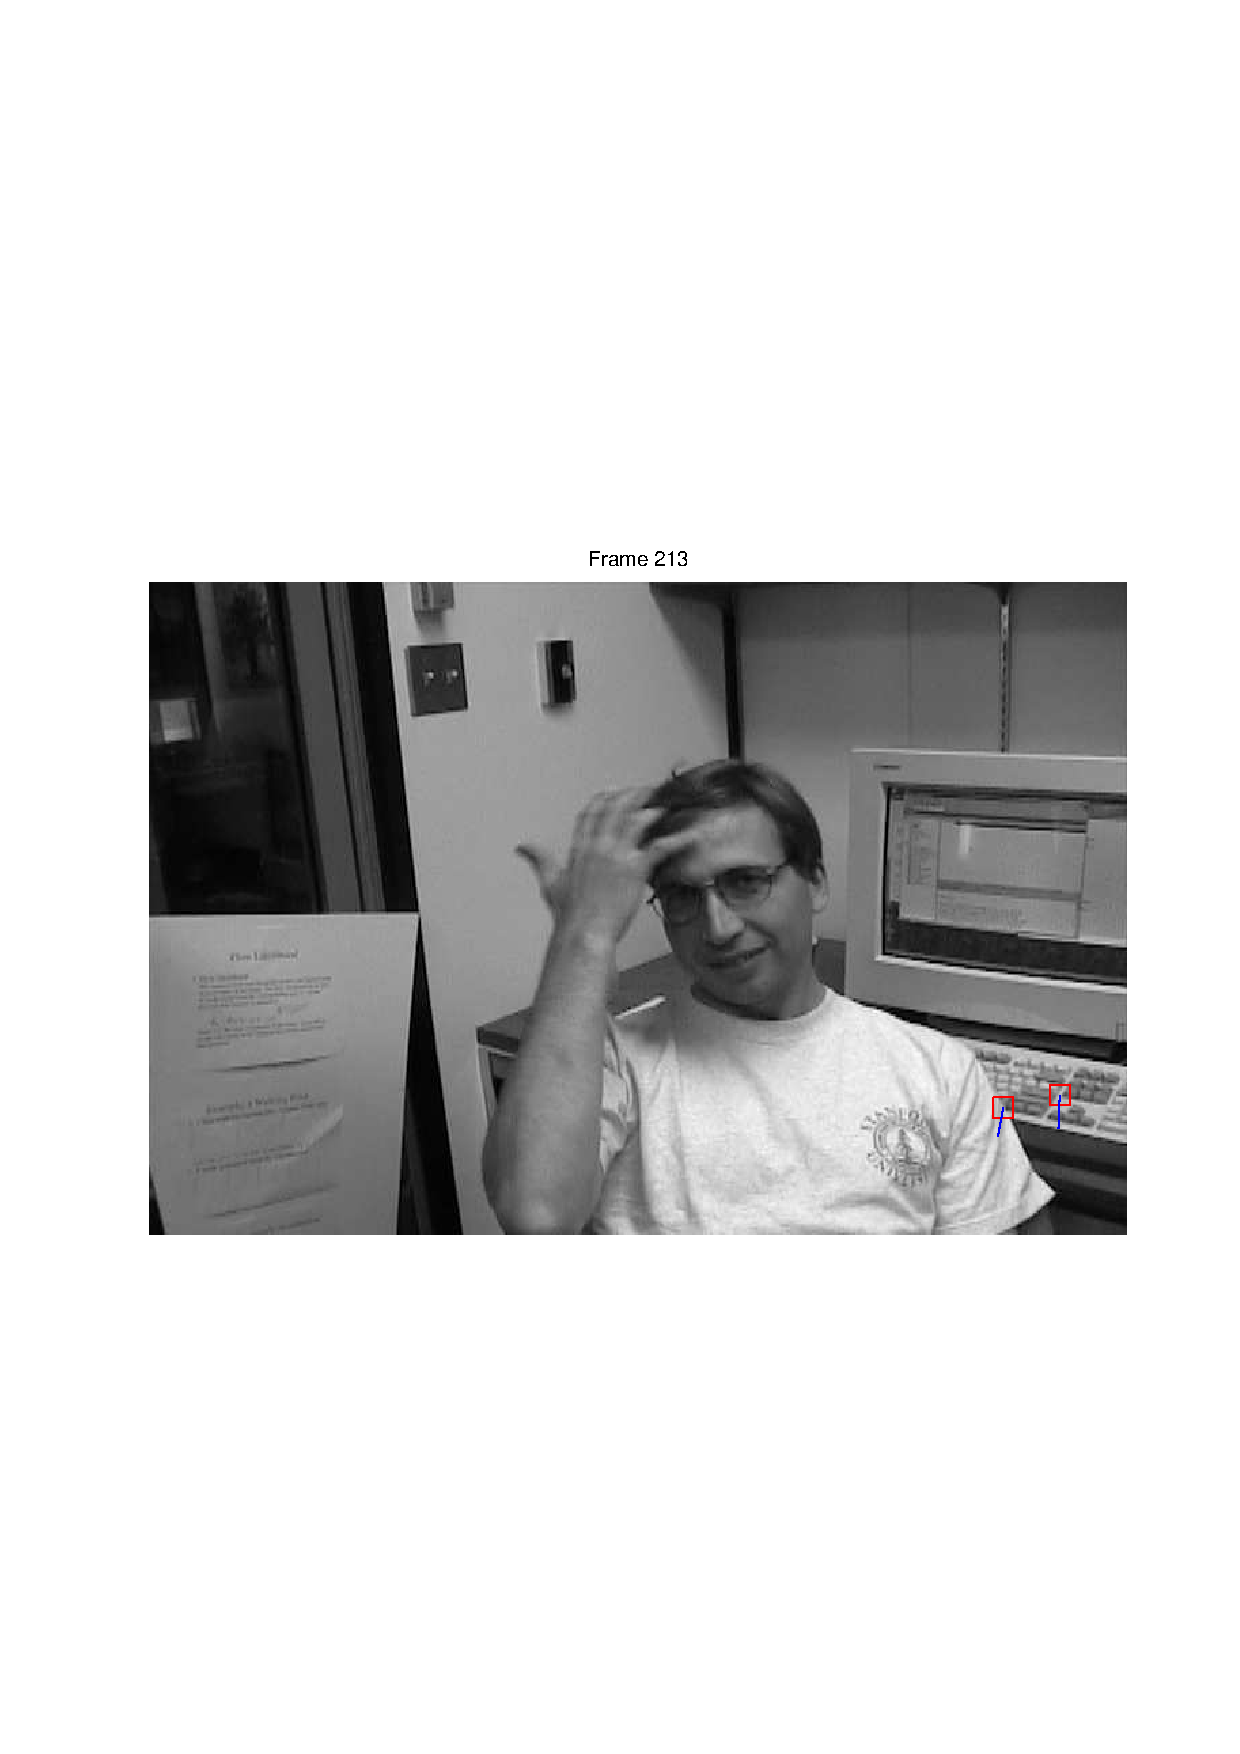
\includegraphics[scale=0.4,trim={70 250 90 250}]{img/tracker_dudekface_213.pdf}
\end{subfigure}
\caption{Frames 1, 10, 100 and 231 from our KLT tracker used on the dudekface image sequence.}
\label{fig:tracker_dudekface}
\end{figure}

\end{document}

